% vim:set textwidth=100:
% vim:set fo+=t:

\documentclass[12pt]{article}

\usepackage{amsmath}
\usepackage[nofiglist,notablist]{endfloat}
\usepackage[usenames,dvipsnames]{color}
\usepackage{color}
\usepackage{authblk}
\usepackage{graphicx}
\usepackage{palatino}
\usepackage[activate={true,nocompatibility},final]{microtype}
\usepackage[super,sort&compress]{natbib}
\pagenumbering{arabic}
\parskip = 0.08in \parindent = 0.0in

% Custom macros for author comments
\newcommand{\Alberto}[1]{\color{ForestGreen}#1\normalcolor }
\newcommand{\Justin}[1]{\color{blue}#1\normalcolor}
\newcommand{\Arijit}[1]{\color{yellow}#1\normalcolor}
\newcommand{\Ken}[1]{\color{red}#1\normalcolor}

\author{Arijit~Roy}
\author{Justin~L.~MacCallum}
\author{Alberto~Perez}
\author{Ken~A.~Dill}
\affil{Laufer Center for Physical and Quantitative Biology\\
    Stony Brook University\\
    Stony Brook, NY 11794-5252.}

\title{Physics-based protein structure prediction and design using the confinement method}

\begin{document}

\maketitle

\begin{abstract}

The calculation of free energy differences is of central importance in the simulation of biochemical
systems.  The computation of the free energy difference between pairs of macromolecule with large
conformational change is particularly a difficult task and computationally expensive with existing
methods. In this work, an improved version of the confinement approach is used to calculate absolute
free energies of bio molecular systems. The method does not require a reaction coordinate or
transition path. It is fast to compute. We show that the method correctly picks out the state of
lowest free energy of a pair of structures having similar sequence but different fold. We also show
using models from CASP9 that the method picks out native-like structures from misfolded or decoys,
provided at least one good structure is in the input set.

\end{abstract}


\section{Introduction}

In computational structural biology there are numerous cases where free energy between well defined
states are necessary. Examples ranges from small to large conformational change of protein due to
ligand binding, change of pH etc \cite{Meirovitch2007}, \cite{Chipot2007}, \cite{Jorgensen2004}. 
Free energy also play an important role in case of protein
folding. The ground breaking work of Christian B. Anfinsen and coworkers showed that the native
structures of small globular proteins have a unique, thermodynamically stable native structure with
their conformation at the global free energy minimum \cite{Anfinsen1973}. Regardless of the starting point or unfolding
it by changing different condition most proteins will finally assume the same structure. It is very
important for proteins to achieve their native conformation since defects in protein folding may be
the molecular cause of a range of human genetic disorder. For example a misfolded protein known as
prion when enters any healthy organism it converts properly folded protein into misfolded one.
Thus, Free energy can also act as a scale to identify between the misfolded and the native state of
the protein. These observations further give free energy a special importance in structural biology.

However, the theoretical calculation of conformational free energy change become difficult if the
states of interest are very different \cite{Meirovitch2007}. In such scenario timescale involved in such tranformation may
be beyond timescale of direct classical molecular dynamics simulation.  Generally, in order to
calculate free energy a pathway or reaction coordinate is created with the intermediate structures.
Method like umbrella sampling \cite{Torrie1977}, thermodynamic integration \cite{Tironi1994} along with classical MD can suffer from
overlap problem and require large computational effort. The idea of reaction coordinate became more
complicated in case of protein folding.  As free energy landscape of the protein folding 
is rough \cite{Dill1997}, \cite{Dill2008}
it can be trapped in a energy well during its visit in the conformational space. Even with the
advanced method like replica exchange molecular dynamics the three dimensional structure may be
trapped in a local minima for a considerable time. Due to various reasons it can also be misfolded
and trapped in a local energy minima. And one can mistakenly identify the misfolded state as the
native state (give the example of human pin1ww domain from Benout Roux and Klaus Schultan).

Calculation of free energy has been successfully attempted by a number of groups \cite{Meirovitch2007}, 
\cite{Ytreberg2006} - \cite{Zheng2008}, . In recent years methods like Refrence system method \cite{Ytreberg2006}, 
Decativated Morphing \cite{Park2008}, Orthogonal Space Random 
Work, Confinement Method have came out for calculation of free energy method. 

Some of the groups
relies on one of the great strength of free energy calculation, that it is a state function and thus
it is independent of path.

In this work we have applied the confinement method which was originally devoled by Tyka et. al. \cite{Tyka2006} and
Cecchini et. al. \cite{Cecchini2009}. The free energy is a state function and thus it can be independent of path. 
Confinement method relies on this fact and uses a thermodynamic cycle where first, non-harmonic degrees of
freedom are removed by applying a series of restraint to the system. Then the free energy of the
remaining harmonic system is obtained using a normal mode calculation and combined with the
non-harmonic part to give the total absolute free energy.  Previously, this method was applied to
calculate the conformational free energy of a 16 amino acid residue peptide, known as BHP.  We have
first reproduced that known result. Then we have applied this method to larger proteins for the
first time. The free energy of conformation of pair of proteins with similar sequence but completely
different fold was calculated. Encouraged by the result, we applied the method of different targets
of CASP9 competition.

%of protein can be obtained to atomic resolution by X-ray crystallography or NMR. Unfortunately, the
%sheer amount of time and economic investment for structure determination cannot keep up with the
%rate at which proteins of unknown structure are sequenced. Therefore, computational models can be a
%good way to bridge the increasing gap between sequence and structure. In this respect CASP
%(Critical Assessment of Structure Prediction) has played a crucial role which is a community wide
%experiments for the protein structure prediction.



\section{Results and Discussion}

\subsection{The confinement method produces correct results in control experiments}

As a first step, we performed several control experiments to verify that our implementation of the
confinement method produces results compatible with previous calculations reported in the
literature.

The method has previously been applied to a 16 amino acid residue $\beta$-hairpin from
protein G, known as BHP \cite{Cecchini2009}. We calculated the free energy difference between two different
conformations of the peptide: (1) the native conformation, called bhp1, with a two-stranded
$\beta$-sheet; and (2) a conformation, called bhp3, which has a three-stranded $\beta$-sheet.
Analysis of long (4 $\mu$s) equilibrium simulations \cite{Cecchini2009},\cite{Krivov2004}  shows that bhp1 is the more favorable
configuration by 1.8 kcal/mol. Using the confinement method, we obtain a value 1.7 kcal/mol, which
is in good agreement with the equilibrium simulations and with previous calculations using the
confinement method \cite{Cecchini2009} (see Supporting Information for further details).

Previous applications of the confiment method have focused on relatively short peptides, up to $17$
residues in length. In this work we apply the confinement method to
larger proteins. On that direction, We first test the confinement method for a chamelon sequence and 
found that it can correctly pick out the prefential structure of the chamelon sequence. Another of the 
applications we explore in the present work is the re-scoring, or
metaprediction, of structures submitted during the Critical Assessment of Structure Prediction
(CASP) experiment (described in detail later). We computed the relative free energies of predictions
submitted during CASP9 10, with the expectation that the most native-like prediction will have
the lowest free energy. As a control, for several targets we also calculated the relative free
energy of the experimental structure (once it was available from the PDB). As
Table~\ref{table:casp_control} shows, in most cases, the confinement method correctly assigns a
lower free energy to the experimentally determined structure than to any of the decoys. 
%Although differentiating between experimentally determined structures and computer generated predictions is
%not a stringent test of a scoring method---for example, examining the residue-residue packing can
%easily distinguish between the two [ref Rosetta Holes]---the results none the less serve as a useful
%"sanity check".

\begin{table}
\label{table:casp_control}
\begin{center}
\begin{tabular}{l l l}\hline
    CASP Target  & PDB Identifier & $\Delta\Delta G_{native \to best decoy}$ (kcal/mol) \\ \hline
     T0531       &    2KJX        &          $12.49 \pm 0.70$ \\ \hline
     T0538       &    2L09        &          $-2.48 \pm 0.47$ \\ \hline
     T0540       &    3MX7        &          $22.00 \pm 0.49$ \\ \hline
     T0559       &    2L01        &          $2.24 \pm 0.24$ \\ \hline
     T0560       &    2L02        &          $22.15 \pm 0.49$ \\ \hline
     T0569       &    2KWY        &          $-9.40 \pm 0.69$  \\ \hline
\end{tabular}
\end{center}
\caption{The confinement method assigns a more favorable free energy to the experimentally
determined structure than to computer-generated predictions. For each target, we examined as many as
five predictions submitted by CASP participants. Positive $\Delta\Delta G$ values indicate that the
experimental structure is predicted to be more favorable than any of the decoys.}

\end{table}


\subsection{The confinement method correctly predicts the structural preferences of chameleon
sequences}

In general, proteins with similar sequences tend to have similar structures. This idea is the basis
of comparative modeling and fold recognition in protein structure prediction. There are, however,
examples---often referred to as chameleon sequences---of proteins with similar sequences that have
remarkably different structures. Orban and co-workers have designed a series of 56-residue proteins
(based on Protein G) that adopt one of two different folds depending on small changes in sequence
(see Figure~\ref{fig:orban}). Sequences that adopt a mixed alpha/beta structure similar to Protein G
are denoted as ``GB'', while sequences that form a three-helix bundle are denoted as ``GA''. One
pair of sequences (GA88/GB88) are 88 percent identical and differ in seven positions. Another pair
(GA95/GA95) are 95 percent identical and differ in three positions. The last pair (GA98/GB98) differ
only in a single tyrosine to alanine mutation.

The fact such small changes in sequence can lead to such dramatic changes in structure is rather
remarkable. Accurately predicting the structural preferences of these structures presents a serious
challenge for computational methods \cite{Alexander2007}$-$\cite{Shortle20009}.

We initially approached this problem by making a model of each sequence with the same backbone
structure as its partner chameleon sequence. For example, we took the sequence of GA88 and built a
model with the same overall structure as GB88. We then used the confinement method to assess the
free energy difference between the experimentally determined structure of GA88 and the model (with
the GA88 sequence and the GB88 structure). The confinement method was able to predict the
conformational preferences correctly for all six sequences (data not shown). There is, however, a
serious problem with this analysis: we are comparing an experimentally determined structure with a
computer generated model. It might be possible that we were able to make correct predictions simply
because artefacts of our modeling procedure always lead to the model having a higher free energy
than the experimental structure.

To avoid this potential problem, we instead computed the relative free energy two different
structural models for each sequence. One model is based on the GA structure and the other on the GB
structure (see Supporting Information for details on the modeling procedure). This is a much more
realistic test of the confinement method's ability to accurately calculate relative free energies.

The results of these calculations are presented in Figure~\ref{fig:orban}. The confinement method
identifies the correct structure for all five sequences. One of the hypothesis for fold switching
of chamelon sequence is that the structural transitions require states with diminished stability.
It is widely believed that if the free energy of the native state and the alternative state is within
 a range of $-5 Kcal/Mol$ then  it can quickly change fold when the stability of the native state 
decreases. The stability of the native state can decrease for a number reason ranging from chemical 
modification, breaking of disulphide bond or mutation as in this case. The free energy differences, that
came out from our calculation ranges from
around 2.9 to 5.7 kcal/mol, which is consistent with the above hypothesis \cite{He2008}, \cite{{Alexander2009}}.

\begin{figure}
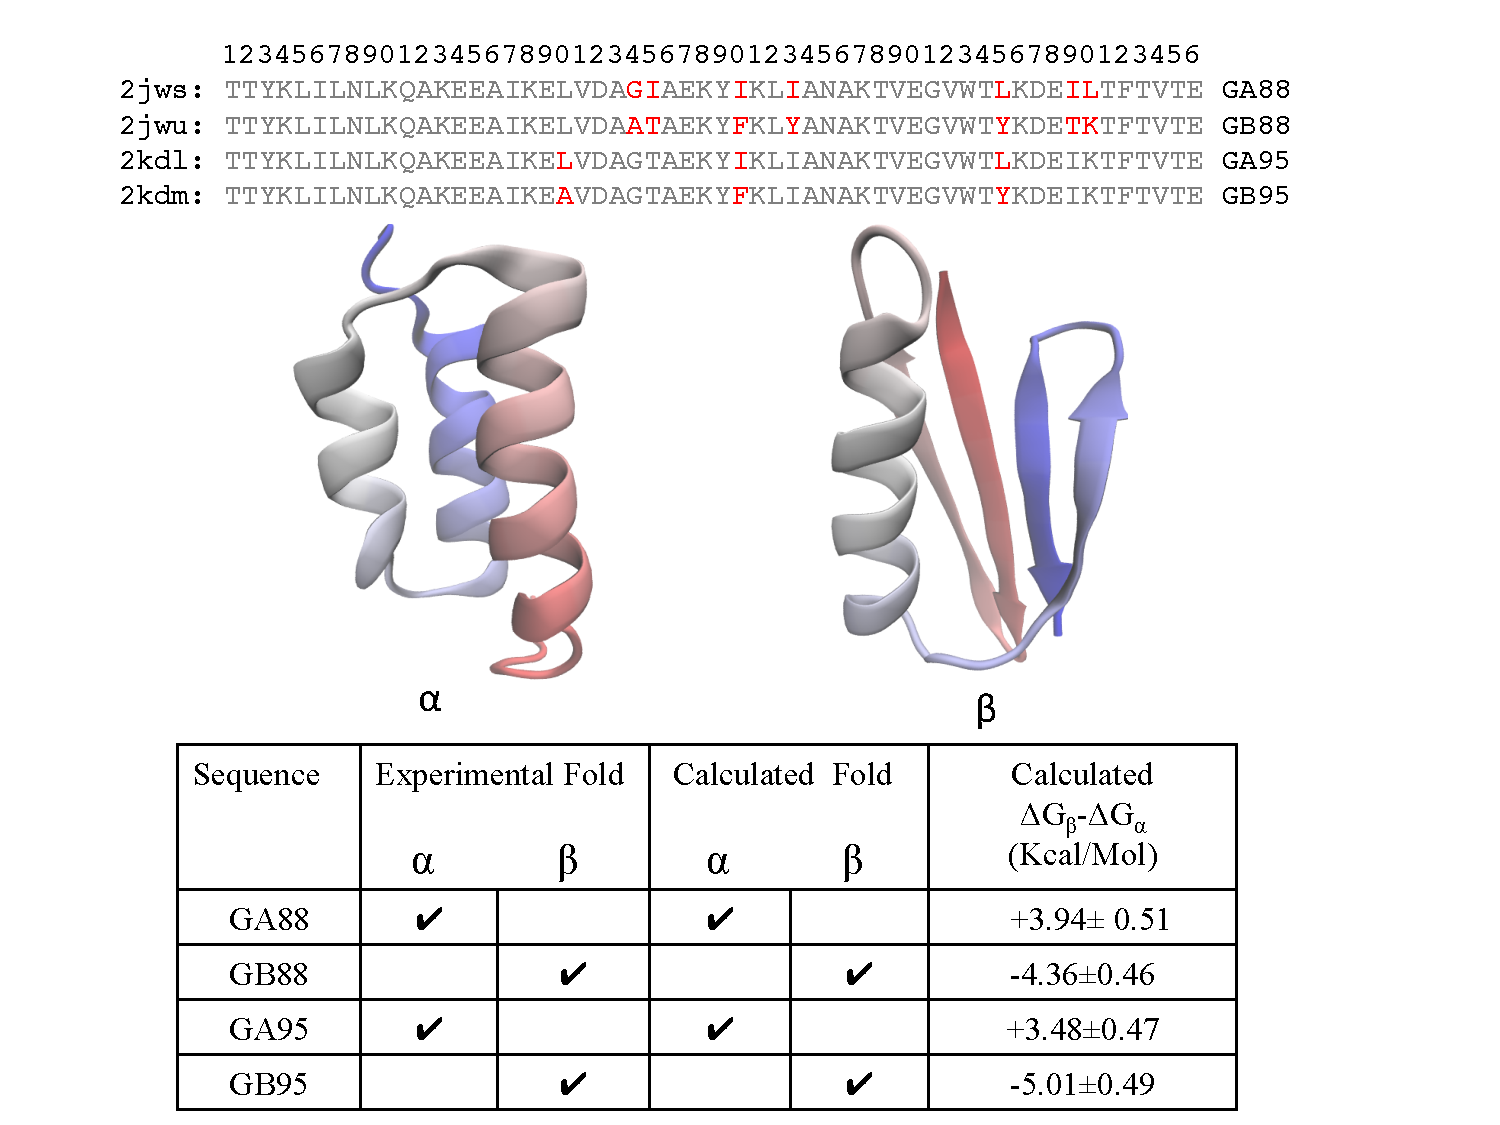
\includegraphics[width=3.5 in,height=4 in]{orban.pdf}
\label{fig:orban}
\caption{The confinement method correctly predicts the structural preferences of six chameleon
sequences. (A) The six sequences used in this study. (B) Each sequence adopts either a Protein
G-like fold (denoted GB) or a three-helix bundle fold (denoted GA). The relative free energies of
the two folds are reported for each sequence.}
\end{figure}

%\begin{table}
%\caption{The confinement method correctly reproduces the structural preferences of a series of
%designed peptides. Each sequence adopts either a Protein G-like fold ($4 \beta + \alpha$) or forms a
%helix bundle ($3 \alpha$).}
%\label{table:orban}
%\begin{center}
%\begin{tabular}{l l l}\hline
%Changes in & $\Delta G$ (kcal/mol)    & $\Delta G$ (kcal/mol)     \\
 %Sequences & ($3 \alpha$ fold)        & ($4 \beta + \alpha$ fold) \\ \hline
%GA95       & $0.000$                  & $2.901 \pm 0.475$         \\
%GB95       & $4.365 \pm 0.460$        & $0.000$                   \\
%GA88       & $0.000$                  & $ 3.941 \pm 0.517$        \\
%GB88       & $5.576 \pm 0.464$        & $0.000$                   \\
%GA98       &  &                           \\ \hline
%GB98       &                          &                           \\ \hline
%\end{tabular}
%\end{center}
%\end{table}


\subsection{The confinement method correctly identifies the most native-like predictions from a
subset of CASP predictions}
\Alberto{Arijit: we need a global table of success, rather than individual tables. The simplest form
    would have 3 columns: name of the PDB, number of structures tested, percent of success of
    picking 1st model}

This method is particularly well suited to pick out the native/native like structure from misfolded or decoys. We have
tested this using different models from CASP (critical assessment of structure
prediction). CASP is a blind test world wide competition in which different groups apply their
methods to predict the 3D structure of proteins given their sequence. This is done with a strict 3
week limit on each target (3 day for servers) and each group is allowed to submit 5 possible
structures (ranked from better to worst). In our role as assessors during the CASP8 and CASP9 \cite{MacCallum2011}
competition we observed no correlation at all between the ordering of structures submited by the
groups and the real ranking compared to an experimental model \cite{Kryshtafovych2011}}. The consequences of this go beyond
those five structures; the deeper meaning is that groups producing ensembles of structures are
generating structures that are better than the ones they submit, but they do not know about it. In
fact, when querrying different groups after the results were known, most groups agree that this is
the case. Beyond the CASP problem, this reflects on the modelers ability to correctly rank order
models in many different environments, from structures for drug design leads to designing more
stable proteins or peptide mimetics such as peptoids. One of the main culprits of this lack of
accuracy is the fact that ranking is often done via a potential energy function, which in many cases
lacks an entropy component. Other initiatives including knowledge based potentials do use some sort
of free energy to rank order, but its accuracy is not enough. Our method provides a physics based
solution to this problem. We have tried two experiments centered on CASP. First we tried to rank
order some structures from the previous CASP9 experiment. Our second test was to participate as a
metapredictor group in CASP10. In both methods, our ranking is determined as a free energy measure,
and it is compared with the ranking given by a geometrical comparison between native and submitted
models called GDT\_TS (Global distance test score \cite{Zemla2003}. 
GDT\_TS represent the average percentage of residues that are in close proximity in two
structures optimally superimposed using four different distance cutoffs (1, 2, 4 and 8 Å).

We have chosen the inital models on which to test the methods based on server groups that have
traditionally done good in past CASP events. There is a high correlation between the structures that
are chosen for this method and its predictive accuracy. In particular, when GDT\_TS scores are below
50, it is difficult for us to say anything about the models. Our approach is simple, with every
subset of structures we choose, we use the confinement method in a pairwise procedure, and then rank
the structures. In all cases, we have calculated the free energy with respect to the native structure either obtained from NMR or 
x-ray crystallography but we do not need to make comparisons to native in order to do rank ordering.

\subsubsection{CASP9}

The question that we want to answer here is whether we can distinguish between native structure and the submitted models? 
%Identifying the native state from a set of models is a very easy test, that most metapredictors
%already handle correctly, but it is also a first proof of principle. 
First we choose a protein BVU3908 from Bacteroides vulgatus whose PDB id and CASP target code are
2L01 and T0559 respectively. The native structure of this 69 residue protein was solved using NMR.
The best predictor group for this target was "BAKER-ROSETTASERVER".
We initlally checked similarity between the models submitted by "BAKER-ROSETTASERVER" and discarded two of them from the 
analysis on the basis of being too similar to some of the other models. The GDT\_TS score and rmsd
values as shown in Figure~\ref{fig:T0559} indicate that the model 1 was predicted correctly, 
whereas the order of model 3 and 5 was wrong. The main difference
between the model 3 and the rest of the model is that the orientation of first alpha helix of model 3 is opposite.
On the other hand, as shown in Figure~\ref{fig:T0559} confine and release method not only can differentiate the native 
structure from the submitted models , it can also correctly rank all the models.  

To further test the method we have taken the example of protein BT2368 from Bacteroides thetaiotaomicron. The PDB id of this 
74 amino acid residue protein is 2L02 and CASP target code is T0560. We have compared the free energy difference between 
the native structure and the two of the five submitted models from the group "Splicer". The remaining three models are discarded as 
again they are similar to the rest of the models. The comparison of GDT\_TS score as shown in 
Figure~\ref{fig:T0560} and published in final CASP result is only for models with residues 3 to 66. In order to keep
consistency, we have also do our analysis with models and crystal structure consisting residues 3 to 66. As expected,
the native state is identified correctly, and the two other models is ranked in the correct order.   

Our next test was between models from the best submissions of different groups. 
For this purpose we have chosen the x-ray crystallographic structure of 
fas apoptosis inhibitory protein molecule whose pdb id and CASP target codes are 3MX7 and T0540 respectively. 
This protein contain 90 amino acid residues with 8 beta strands. We have chosen best models from groups 
"LTB" and "Mufold" for our analysis, which are labelled as Model 1 and Model 2 in Figure~\ref{fig:T0540}. 
As presented in  Figure~\ref{fig:T0540} we found that this method is able to correctly order the models which matches 
with the GDT\_TS score. 

There are however some instances where the method can fail, specially when GDT scores are
very close. We have found this for an engineered protein from Asr4154 protein (PDB ID: 2L09 and CASP Target T0538).
This protein contains 54 amino acid residues with three alpha helixes and two very short beta strand. 
The model that is closest to the native structure was generated by the group PconsR with a GDT\_TS value of 96.23.
We have also considered one model from group "Shell" (GDT\_TS = 90.09) and "FOLDIT" (GDT\_TS = 86.32) for our analysis along with
the native crystal struture. The models from PconsR, Shell and FOLDIT are labelled as model 1, model 2 and model 3 
respectively in Figure~\ref{fig:T0538}. As presented from Figure~\ref{fig:T0538}, one can found that the 
model from PconsR has lowest free energy value, making it a more stable structure. Although ranking of the other models
remain consistent, it may happen that the theoretical model produced by the group "PconsR" much more stable than the 
crystal structure. This is particularly difficult target for rank ordering as all the models those are considered for this 
calculation are within RMSD values of 2.6 \AA.   

There is another instance where this method fails. This is the case of solution NMR structure of a domain of adhesion exoprotein 
from Pediococcus pentosaceus. The
pdb id and CASP code of this 79 residue protein are 2KWY and T0569 respectively. We have compared the native structure with the
best model structure submitted for this target in CASP9. This model structute was submitted by the group " Mufold". ALl the
five model structures submitted by this group was found to be close. Thus we proceed by comparing only the native structure and
the best predicted model of this target. Visualization upon superimposition of two structures reveals that
the difference between the two structure is at the region consist of residues 48 to 65, where model1 is much more disordered compare to the
native structure(see Figure~\ref{fig:T0569}) . Other regions look similar for both the cases with of model1 is within 2.6 \AA
rmsd value of the native structure. In this case we found that the confinement method predict that the predicted model is stable than the
native structure with a free energy difference of $9.4 \pm 0.7$ Kcal/Mol.

\subsubsection{What can we say about low resolution models?}

We mentioned earlier that our predictive abilities are greatly decreased with low model qualities. It is
better to have atleast one good model to pick out the native/native like structures from the rest of the decoy. 
In oorder to test this hypothesis we performed another test with target T0531 of CASP9, in which we compared the crystal 
structure to five models from the MUFOLD server. The pdb id of this extracellular domain of the jumping translocation 
breakpoint protein is 2KJX and the CASP target code is T0531.
Looking at Figure~\ref{fig:T0531} shows: 1.) native is correctly
identified as expected and 2.) Surprisingly there is a high level of correlation between the GDT
ranking and the free energy ranking, only two structures with GDT\_TS score less than  35  are ordered
incorrectly. It is worth to note that models 2 and 3 have the same GDT and very different free
energies, meaning that the actual ordering could change a lot \cite{Perez2012}.

\subsubsection{Difficulty in CASP Experiments}

It is often difficult to model CASP targets using confinement and release method. There are many cases,
where the sequence of a particular target are trimmed during actual result presentation. This is illustrated
with the crystal structure of the leucine zipper domain of cGMP dependent protein kinase I (pdb id: 3NMD
and CASP9 code: T0605) as shown in Figure~\ref{fig:T0605}. The actual CASP 9 target consisted of 72 amino acid residues, but
as only 18-66 amino acid residues could be detected in actual crystal structure of this protein, the final result was trimmed 
with respect to that crystal structure with 49 amino acid residues which consist of a single alpha helix. The amino acid residues 18 and 66 are shown in
three models submitted by the group "Baker". It is important to note that blind prediction of model ranking on the basis of free energy can be hugely 
affected in such scenario as the only major difference between those models are the trimmed parts, specially the region consisting residues 1-18.    


\subsubsection{Can confinement method perform better quality assessment in protein structure prediction ?}
A part of CASP experiment is dedicated to the assessment of the quality of predicted model \cite{Kryshtafovych2011}. 
Most of the top performing group in this catagory use consensus approaches for quality assessment \cite{Wang2011}.
A review of CASP9 quality assessment also pointed out that the method which are based on clustering technique perform
much better compare to those methos which are based on analysis of individual model \cite{Kryshtafovych2011}. 
In this background we try to answer, whether confinement method can do better quality assessment compare to the best performing
group (MUFOLD-WQA) in this catagory.
We have again picked up the CASP taget T0538 to answer this question. We have chosen the Model 3 submitted by PconsR (GDT\_TS = 96) 
and model 5 from the MULTICOM-NOVEL ( GDT\_TS = 83). Both are server predicted model and they were further used for quality assessment 
by the group MUFOLD-WQA \cite{Wang2011}. It is important to note that the model from PconsR was most accurate predicted model for this 
target and the model from MULTICOM-NOVEL was predicted as best by the quality assessment experiments of MUFOLD-WQA. 
Our free energy analysis we have shown that model from Pconsr is better than the model from 
MULTICOM-NOVEL $(\Delta \Delta G (Model\_Pconsr - Model\_MULTICOM-NOVEL = -8.2 Kcal/Mol)$, which   
matches well with the GDT\_TS score. On the other hand the MUFOLD-WQA predicted the ranking in the reverse order. 
There is no doubt that the consensus approaches can predict the model quality in a faster manner. But we expect that confinement
approach can predict the model quality in a relatively expensive but much accurate way. 

\Arijit{Will upload the result from Target 560 once cluster is back.}


\subsubsection{CASP10}

We participated in CASP10 as a metapredictor group. Given the tigh schedule of the CASP competition,
we only attempted proteins under 100 residues in length. Our main problem during this part of the
competition. was that proteins were trimmed from the actual calculation.
%\Alberto{Justin,Arijit: Probably should not comment on metapredicting since we were not able to do
%    good due to the trimming factor. Instead, we should move forward with Justin's idea of using
%    structures that other meta predictors did badly at. What stage is that in?}

\section{Conclusion}

Proteins are essential parts of organisms and participate in virtually every process within living cells. 
In order to understand different functions of proteins, detect diseases caused by them and design more efficient drugs 
it is often useful to have the three dimensional structure of the protein. Experimental studies using NMR and X-ray crystallography is 
not enough to detect large number of structures. In recent past there are number of studies directed towards understanding protein 
structure using theoretical tools. Experimentally, it is relatively easy to identify the native structure from the data obtained 
from x-ray crystallography or NMR. On the other hand using theoretical tools it is often difficult to identify the native structure 
using both physics based methods and knowledge based method. In order to rank structure from the available data, some groups use 
clustering algorithms and the structure of the
most populated cluster is picked out as the most probable structure. However, it may happen that the structure may be trapped and 
spend most of its time in a kinetic trap, which may give a wrong interpretation of the clustering result. On the other hand, some groups
also depend on potential energy function to pick out their best structure. In this paper, we have used a free energy method to identify
the native/native like structure. First, we have tested this method for a chameleon sequence, which has a $95$ percent sequence identity
but one of them has a $3 \alpha$ structure and another one has $4 \beta + \alpha$ structure. Using the current method, we can found that 
the native structure always has most stable structure. We have also tested this method for different targets of CASP experiments. We found
that in most cases, it can pick out the native/native like structure in terms of lowest free enrgy value. 

However, there may be some limitation of this method in terms of size of the protein molecule. The normal mode analysis may not be
accurate for proteins larger than 100 amino acid residues. This can be approximated by removing the hydrogen molecules from 
the system. 
The method can be also give wrong result if all the models in the decoy are very poor. It may also be difficult to rank structures if 
all the structures are very very close to the native structure. But that does not matter at all as our main aim is to differentiate
between the good and the bad structure. In this article we have extensively tested this method using examples from CASP experiment.
This method can be computationally expensive in actual CASP experiment if one want rank thousands of submitted models in CASP 
experiments. However, in real life experiment with a particular target this method can give accurate result. The important 
fact about Confinement method is that all the part of the calculation can be done independently. We have mostly carried out 
our calculation with Amber program \cite{Case2005} in GPU computer. With a avarage 56 residue we found that it take only 4 hour to complete 
20 ns of the confinement step. So, with available computer power this method will be easy to use.  
 
This method can be further used for calculating free energy due to very large conformational change. Another application may be
for the case of ligand binding. It can also be used to distinguish the most stable structure during protein design. Another, important
application may be to study the protein folding kinetics, specially to study the phi value analysis.            


\section{Method}

The confinement method has been described in details in ref. by Tyka et.al. \cite{Tyka2006} and 
Cecchini et. al. \cite{Cecchini2009}. The basic approach of confinement approach is same in both
these paper. However, there are some technical differences. Here we briefly describe what we follow
to compute free energy $\Delta G_{AB}$ between A and B
conformation of the protein.

\begin{enumerate}

\item  We first minimized both the conformation, A and B. These minimized conformation(A* and B*) 
       are the reference conformation of that state

\item Backbone dihedral angle of both the full protein is restrained by a harmonic potential. This is required to keep
    the configurational state of the protein. This approach is particularly important, so that the any misfolded part 
    of the protein does not chage its configuration. 

\item  The free energy is calculated using a thermodynamic cycle. The first part of this approach is the confinement, where
       the state A and B are confined to the reference state A* and B*. This is done gradually by applying larger and larger
       harmonic restraint on all the atoms of the biomolecule. This is done by running 21 molecular dynamics simulation 
       each of 20 ns long, where the harmonic restraint constant was varied from 0.00005 to 81.92 untill the free and the 
       restrained state overlap well. The final restrained state was chosen so high so that the rotational contributional 
       of the protein frozen out and only remaining contribution remain that of vibrational free enrgy. The fluctuation from
       the reference structure was recorded and the free energy is calculated using a numerical
       approach developed by Tyka et. al. \cite{Tyka2006}. The confinement free energy calculated in this way recorder as 
       $\Delta G_{A,A*}$ and $\Delta G_{B,B*}$ as shown in Figure~\ref{fig:method}.     

\item  Finally the thermodynamic cycle is closed by calculating the free energy between the final
       restrained state A* and B* using normal mode analysis or quasiharmonic analysis. The free energy calculated in 
       this way is shown as $\Delta G_{A*,B*}$ in Figure~\ref{fig:method}.

\item  The full free energy, $\Delta G_{A,B}$ between the two state A and B is calculated using the equation 
       $\Delta G_{A,B}$ = $\Delta G_{A,A*}$ - $\Delta G_{B,B*}$ + $\Delta G_{A*,B*}$  

\end{enumerate}

In all the calculation amber 10 program is used with ff99SB with GB/SA implicit solvent.  



\begin{figure}
\begin{center}
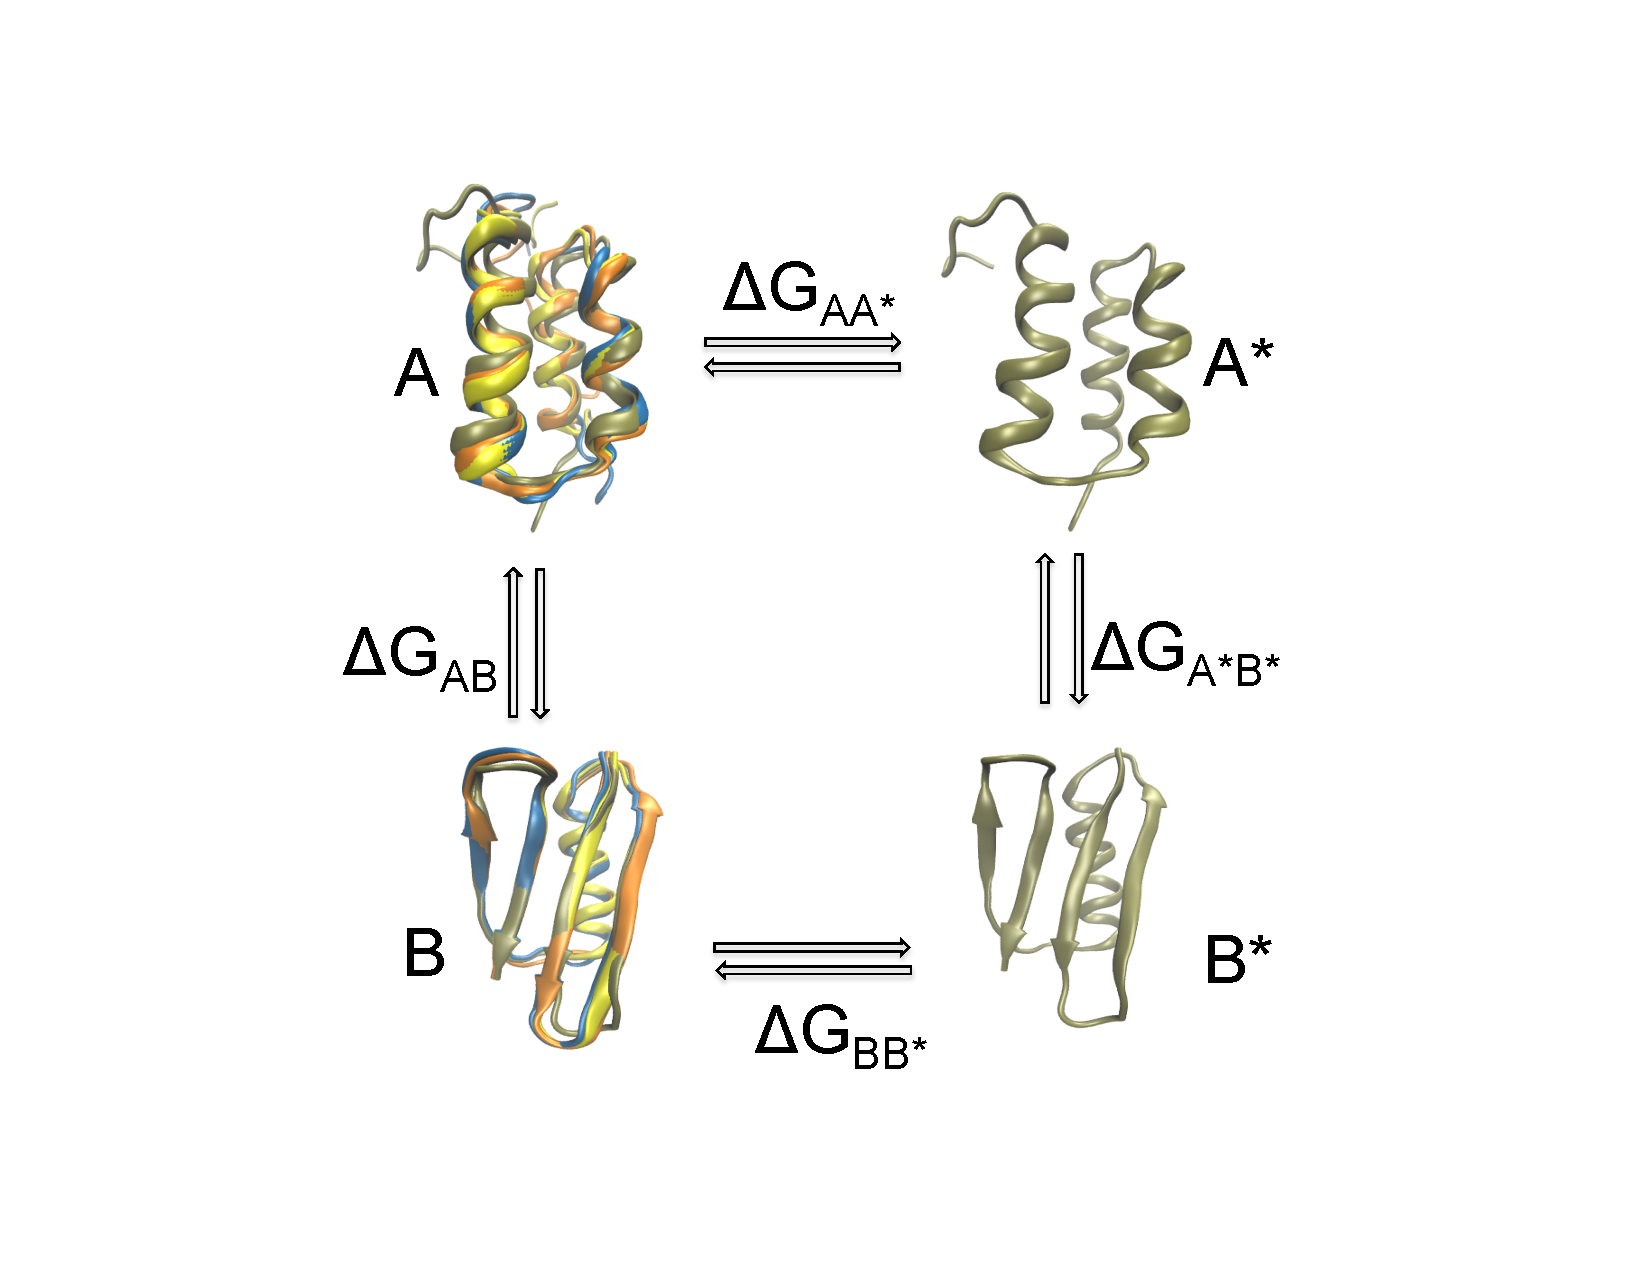
\includegraphics[width=3.5 in,height=3.5 in]{method.pdf}
\end{center}
\caption{Graphical representation of the thermodynamic cycle involving confinement method.}
\label{fig:method}
\end{figure}


\begin{figure}
\begin{center}
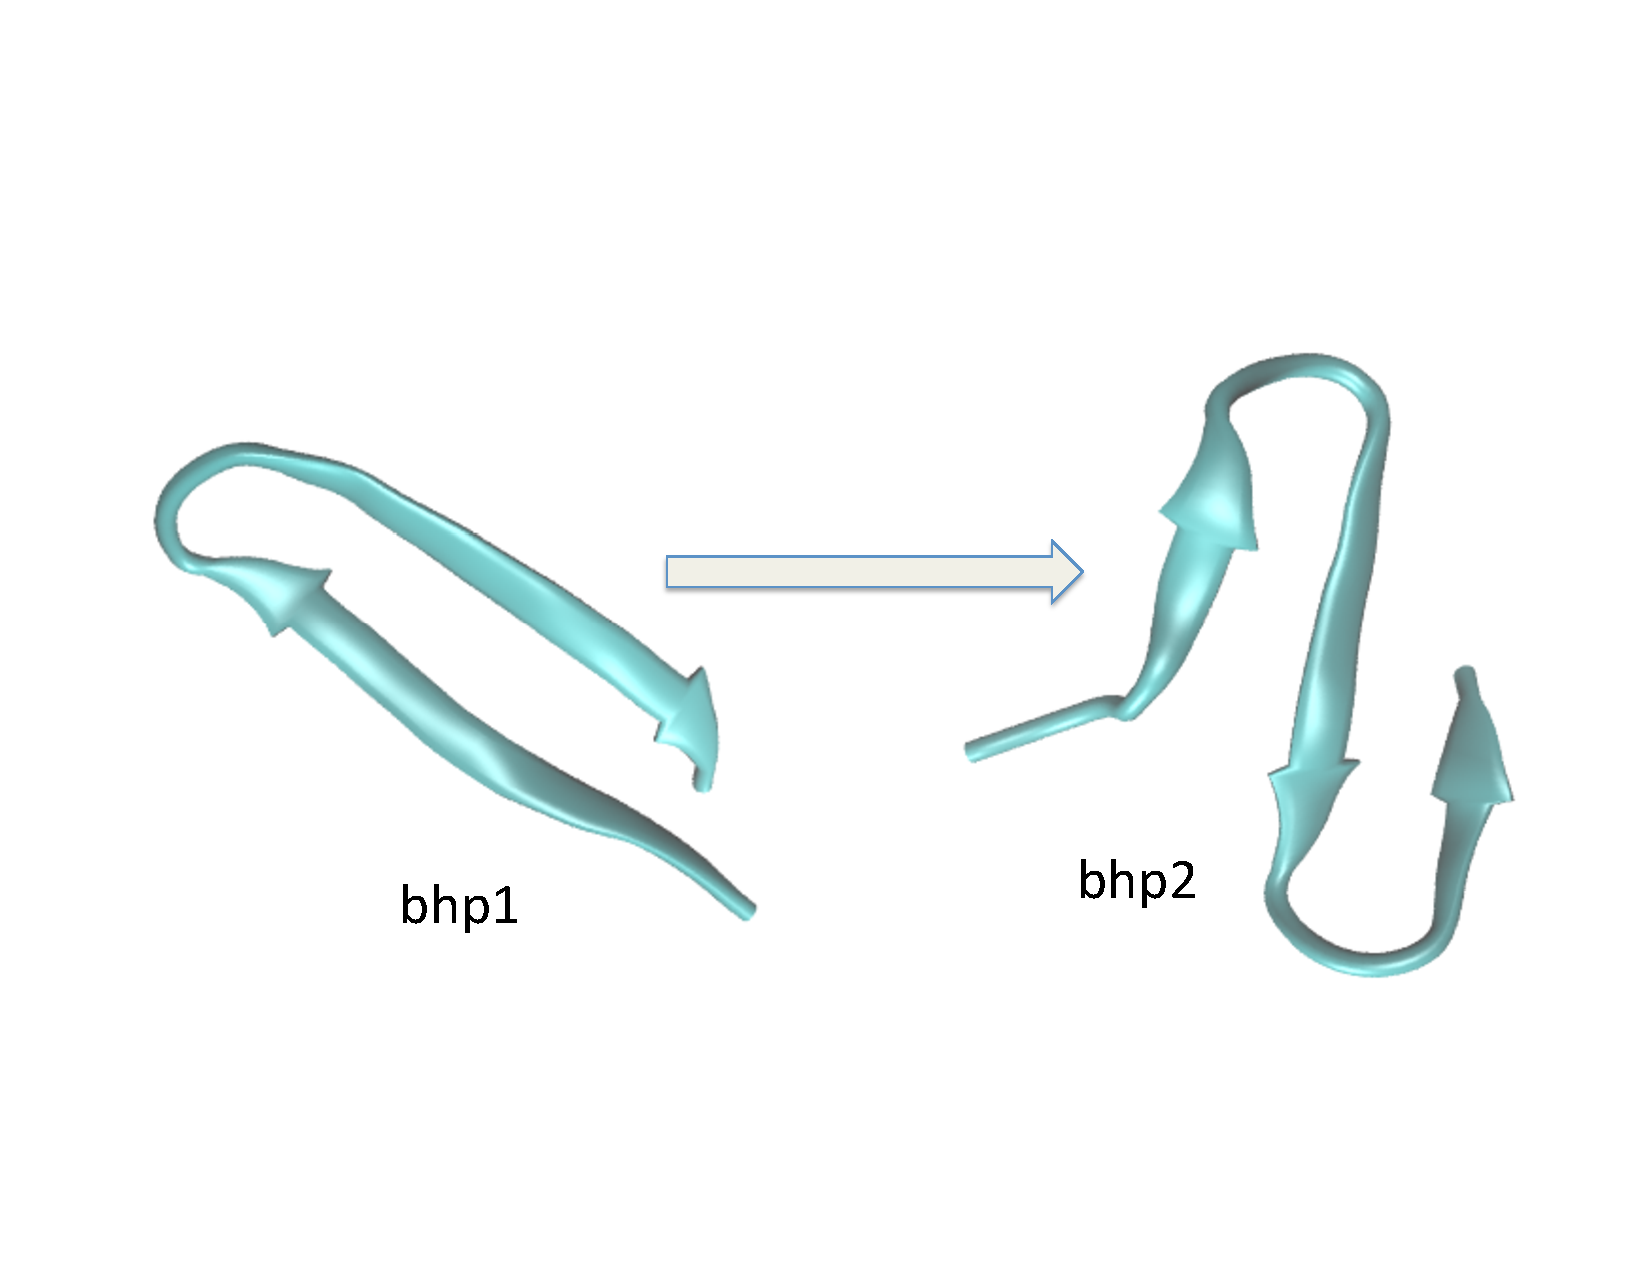
\includegraphics[width=3.5 in,height=3.0 in]{bhp.pdf}
\end{center}
\caption{Two conformations from $\beta$ hairpin from protein G, bhp1 and bhp2. The two stranded $\beta$ sheet, bhp1 is the native structure and the three stranded $\beta$ sheet is known as bhp3.}
\label{fig:bhp_conf}
\end{figure}

\begin{figure}
\begin{center}
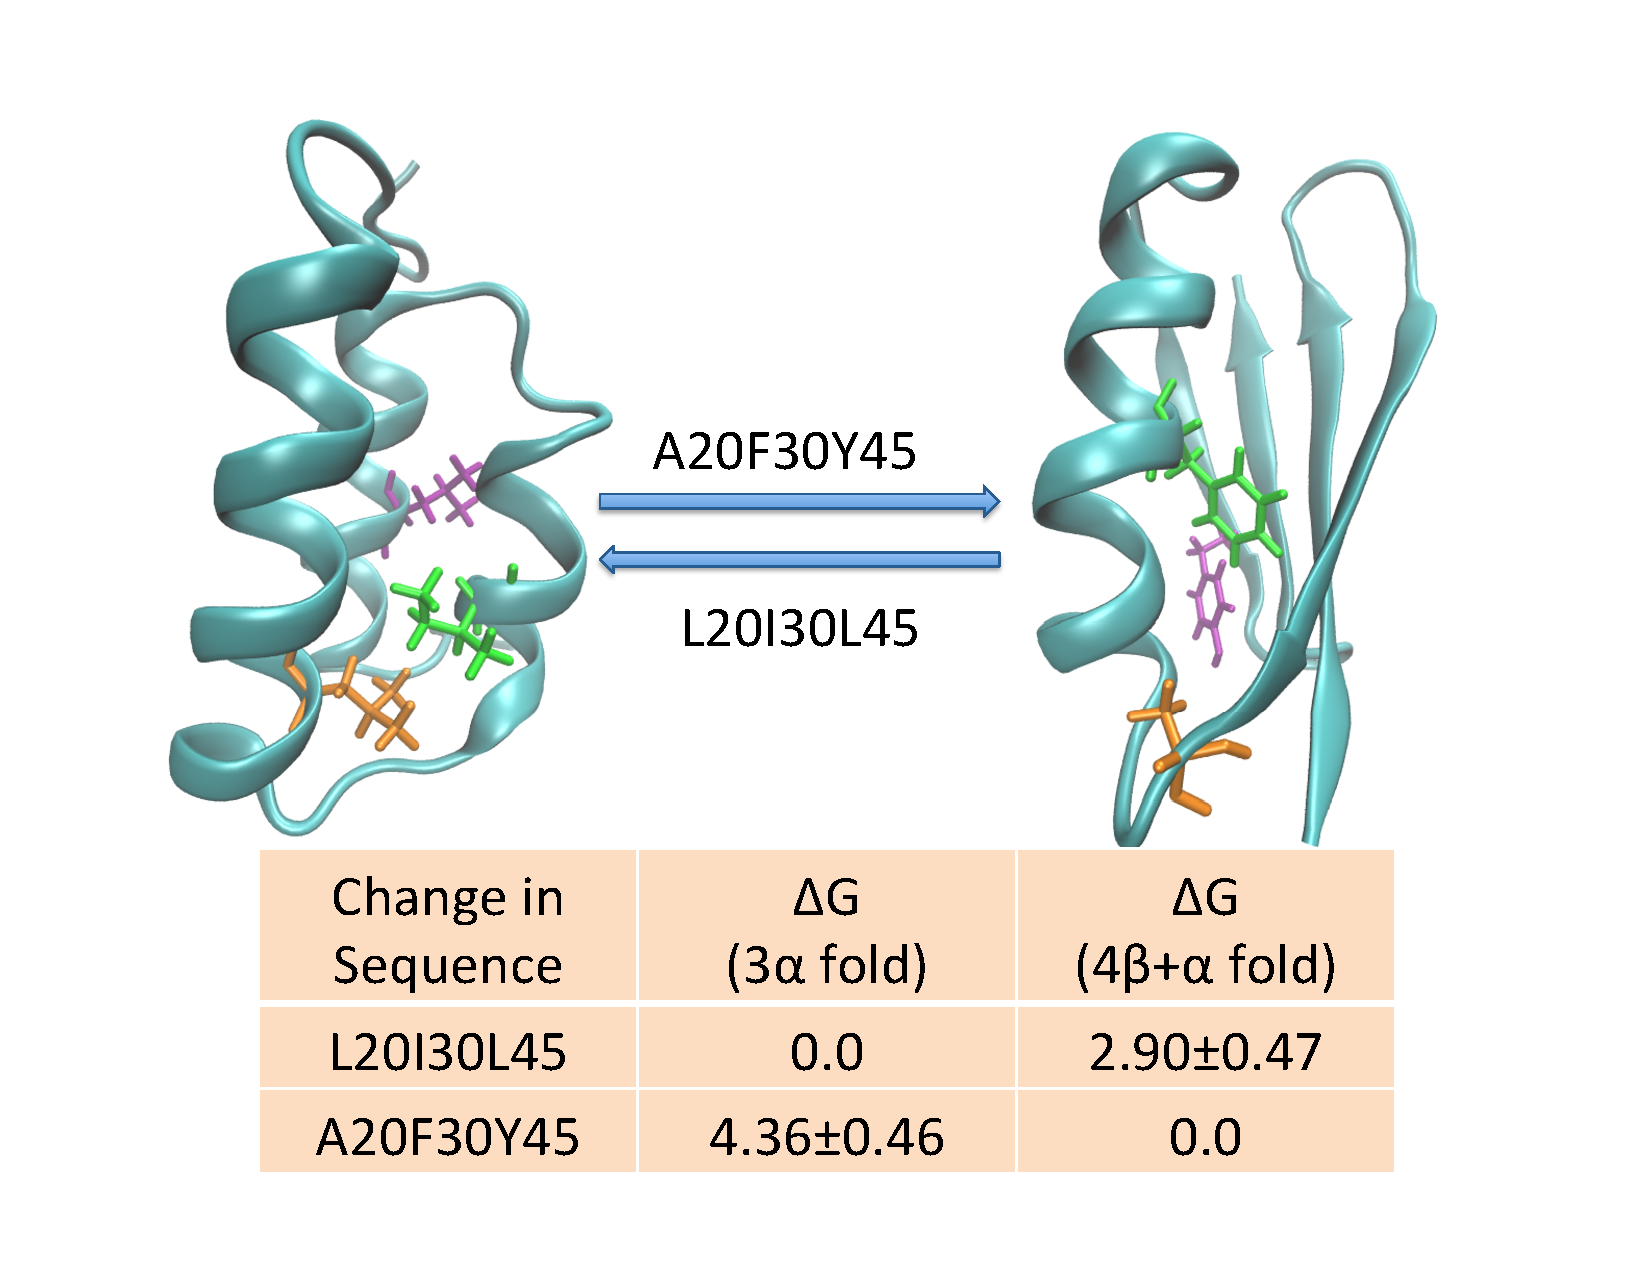
\includegraphics[width=3.5 in,height=3.0 in]{G95.pdf}
\end{center}
\caption{Two protein with 95 \% similar sequence but different folds}
\label{fig:G95}
\end{figure}

\begin{figure}
\begin{center}
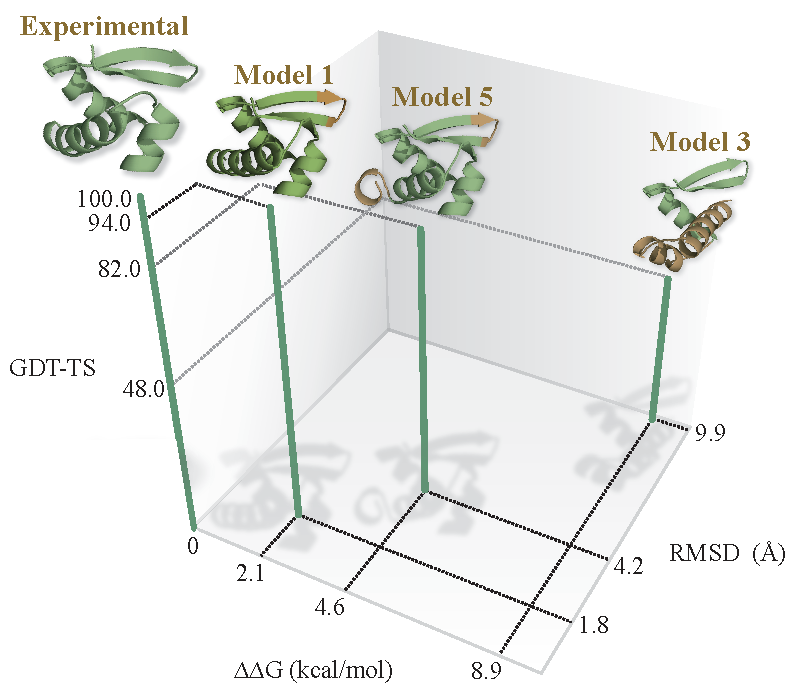
\includegraphics[width=3.8 in,height=3.0 in]{T0559.pdf}
\end{center}
\caption{The native and three submitted model structure, along with their GDT\_TS, RMSD and relative Free energy values 
of protein BVU3908 from Bacteroides vulgatus (PDB id: 2L01 and CASP code: T0559).}
\label{fig:T0559}
\end{figure}

\begin{figure}
\begin{center}
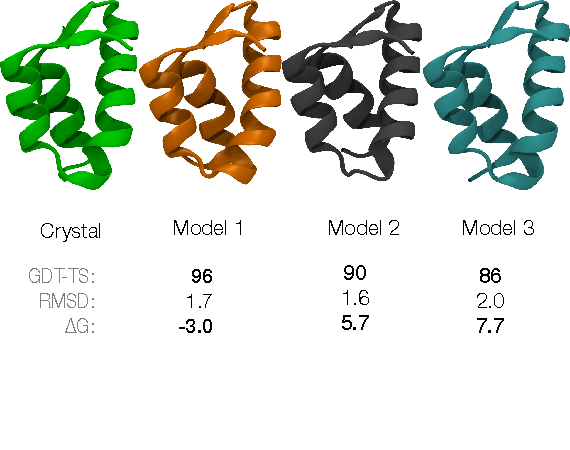
\includegraphics[width=3.8 in,height=3.0 in]{T0538.pdf}
\end{center}
\caption{The native and three model structure of engineered protein from Asr4154 protein (PDB ID: 2L09 and CASP code:T0538). The model 1,2 and 3 are
from the group PconsR, Shell and FOLDIT respectively.}
\label{fig:T0538}
\end{figure}

\begin{figure}
\begin{center}
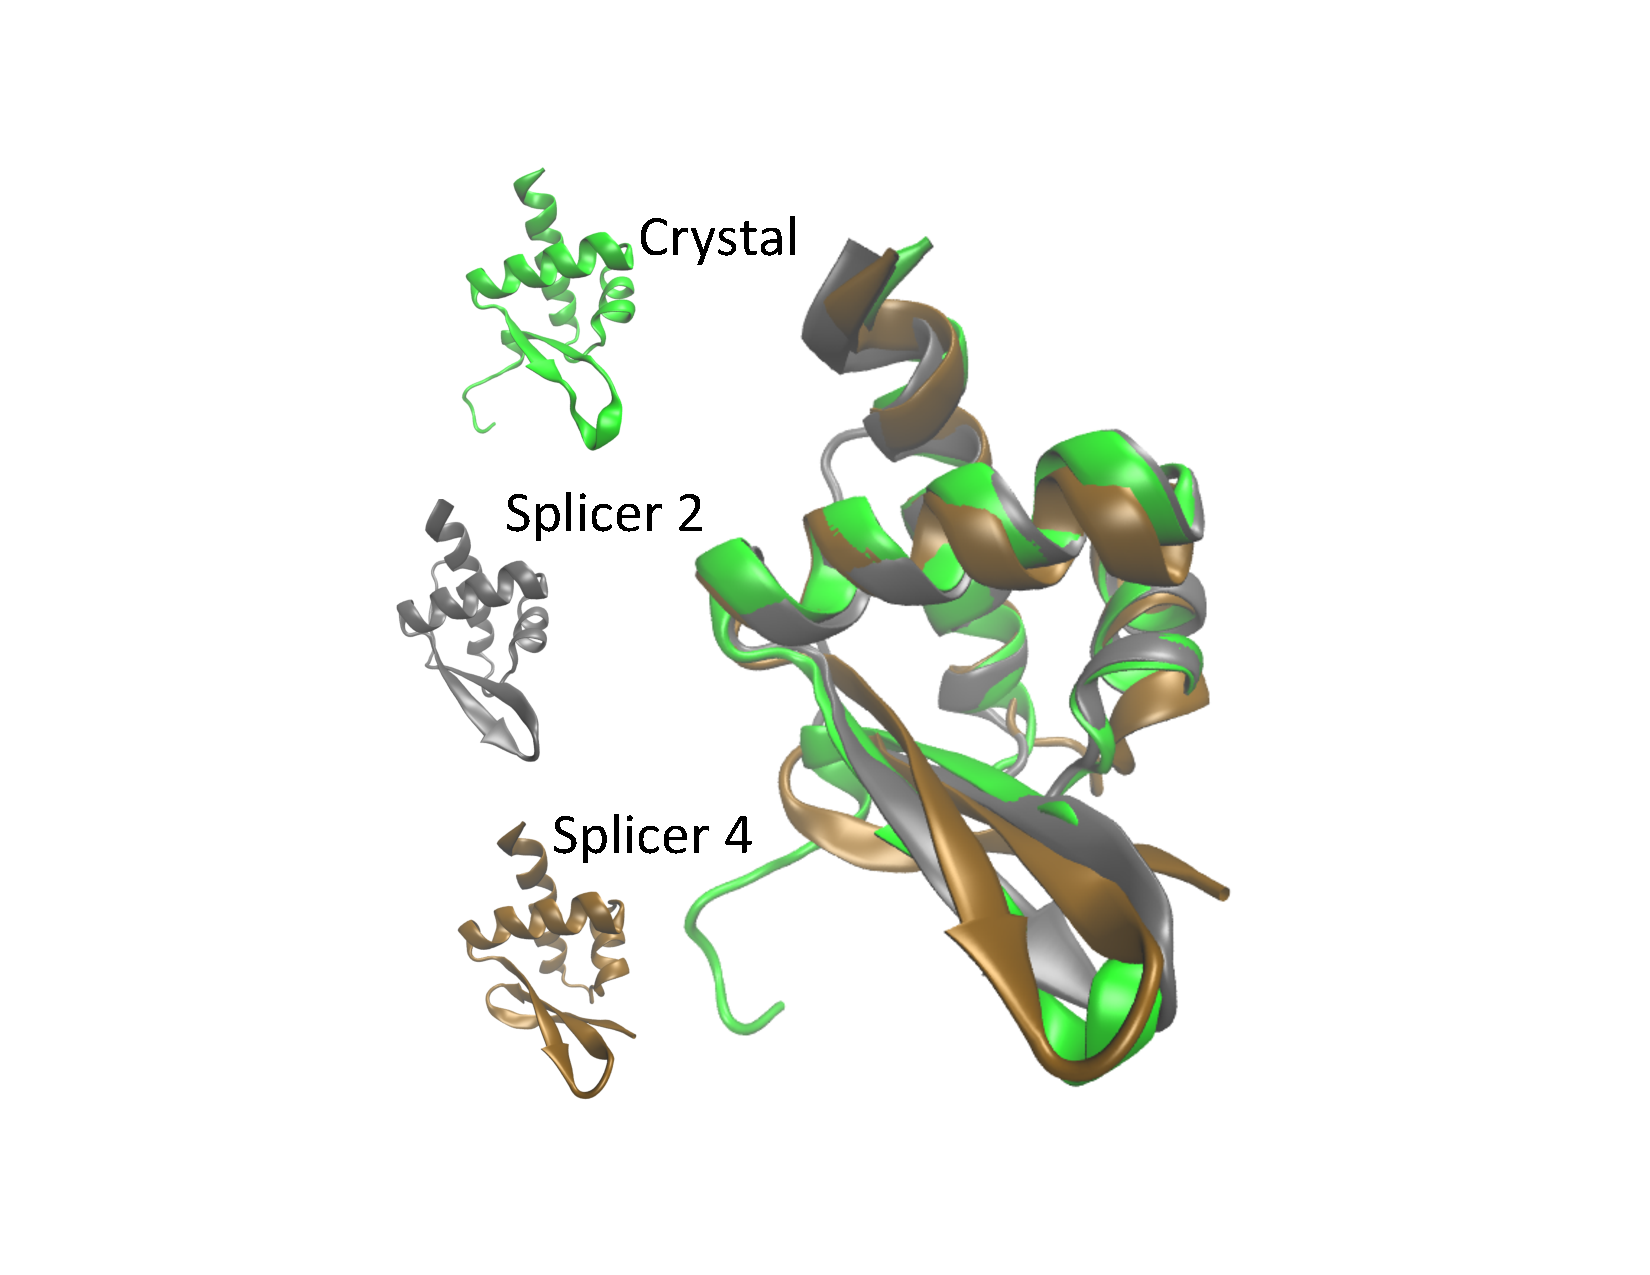
\includegraphics[width=3.5 in,height=3.0 in]{T0560.pdf}
\end{center}
\caption{Native and two model structure of protein BT2368 from Bacteroides thetaiotaomicron (pdb id: 2L02 and CASP code: T0560). The two models
were from the group "Splicer".}
\label{fig:T0560}
\end{figure}

\begin{figure}
\begin{center}
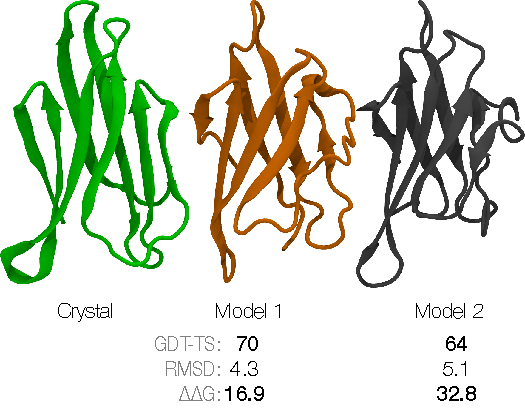
\includegraphics[width=3.5 in,height=3.0 in]{T0540.pdf}
\end{center}
\caption{X-ray crystallographic structure and two submitted models of fas apoptosis inhibitory protein (pdb id: 3MX7 and CASP code: T0540). 
Model 1 and Model 2 in this analysis were submitted by the group LTB and MUFOLD respectively.}
\label{fig:T0540}
\end{figure}

\begin{figure}
\begin{center}
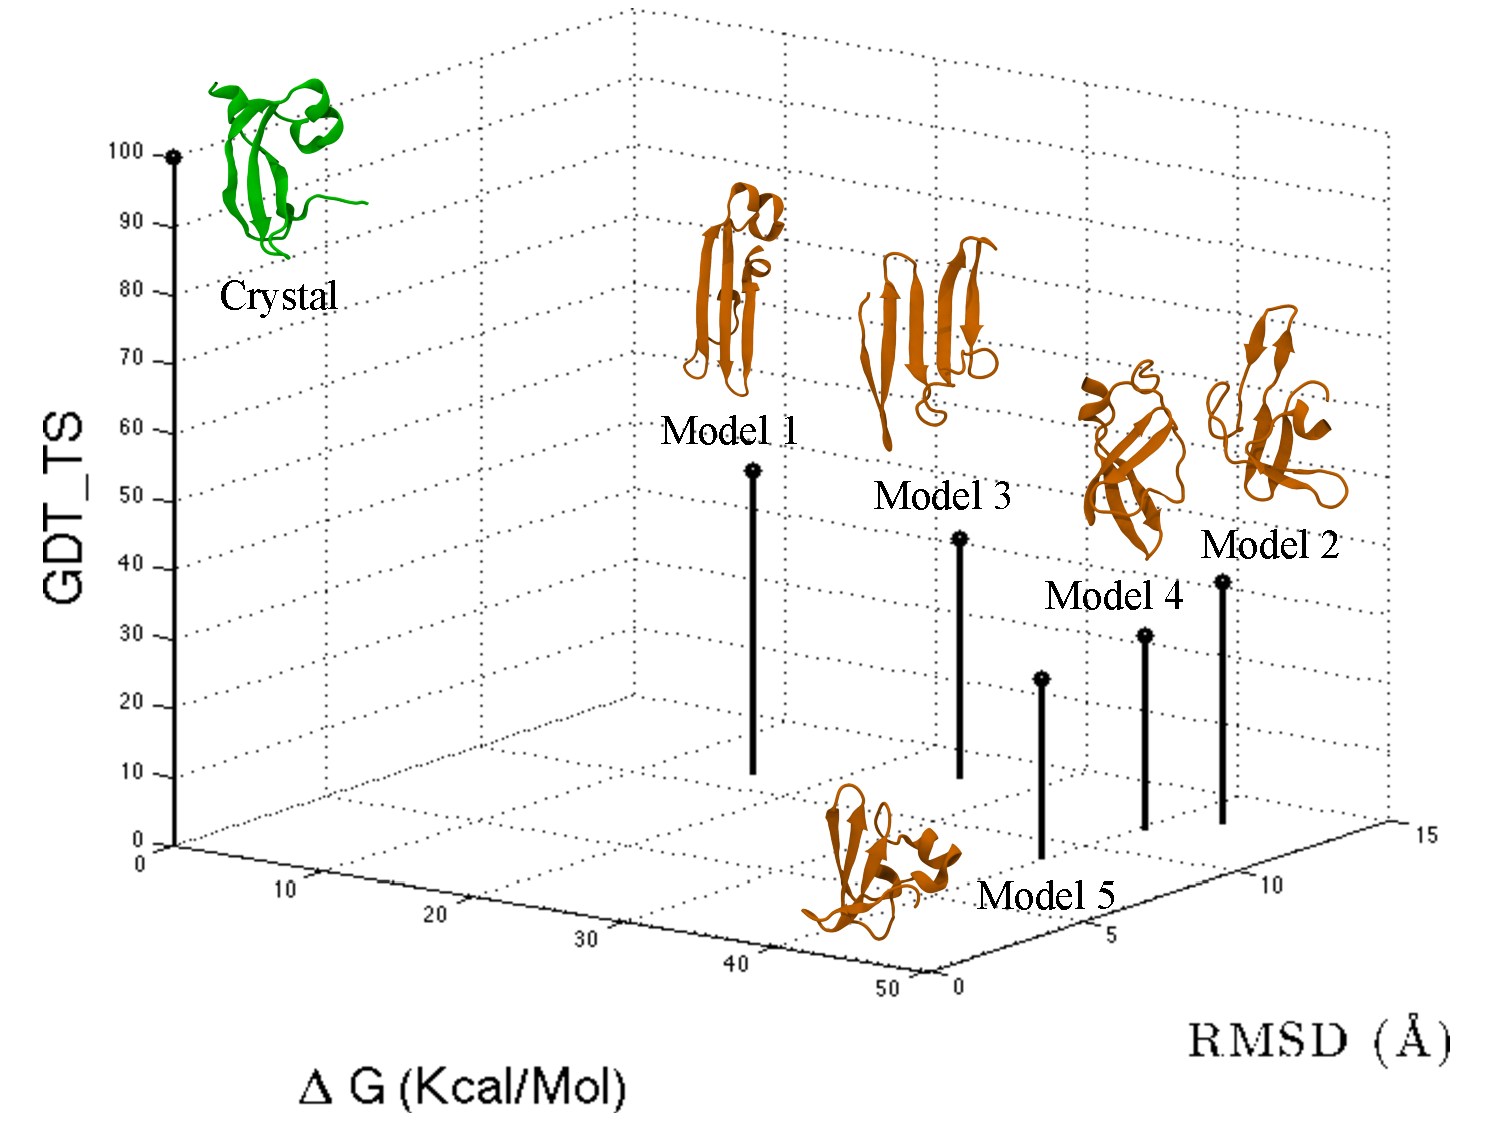
\includegraphics[width=3.5 in,height=5.7 in]{T0531.pdf}
\end{center}
\caption{The native structure and 5 models of extracellular domain of the jumping translocation
breakpoint protein (pdb id: 2KJX and the CASP code: T0531).}
\label{fig:T0531}
\end{figure}

\begin{figure}
\begin{center}
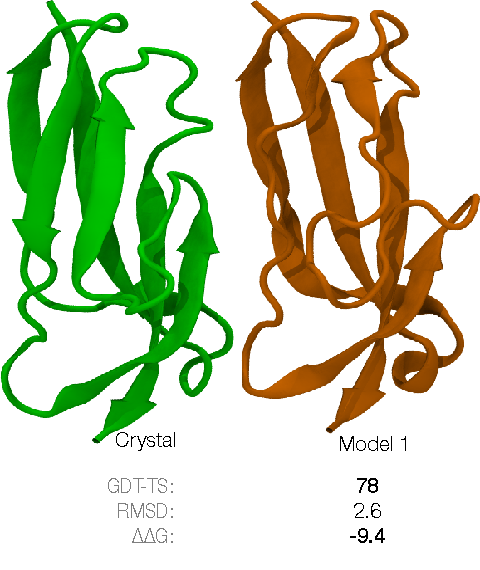
\includegraphics[width=3.2 in,height=3.8 in]{T0569.pdf}
\end{center}
\caption{Native and best model structure of a domain of adhesion exoprotein from Pediococcus pentosaceus (pdb id: 2KWY and CASP code: T0569).
The best model was from the group "Mufold".}
\label{fig:T0569}
\end{figure}

\begin{figure}
\begin{center}
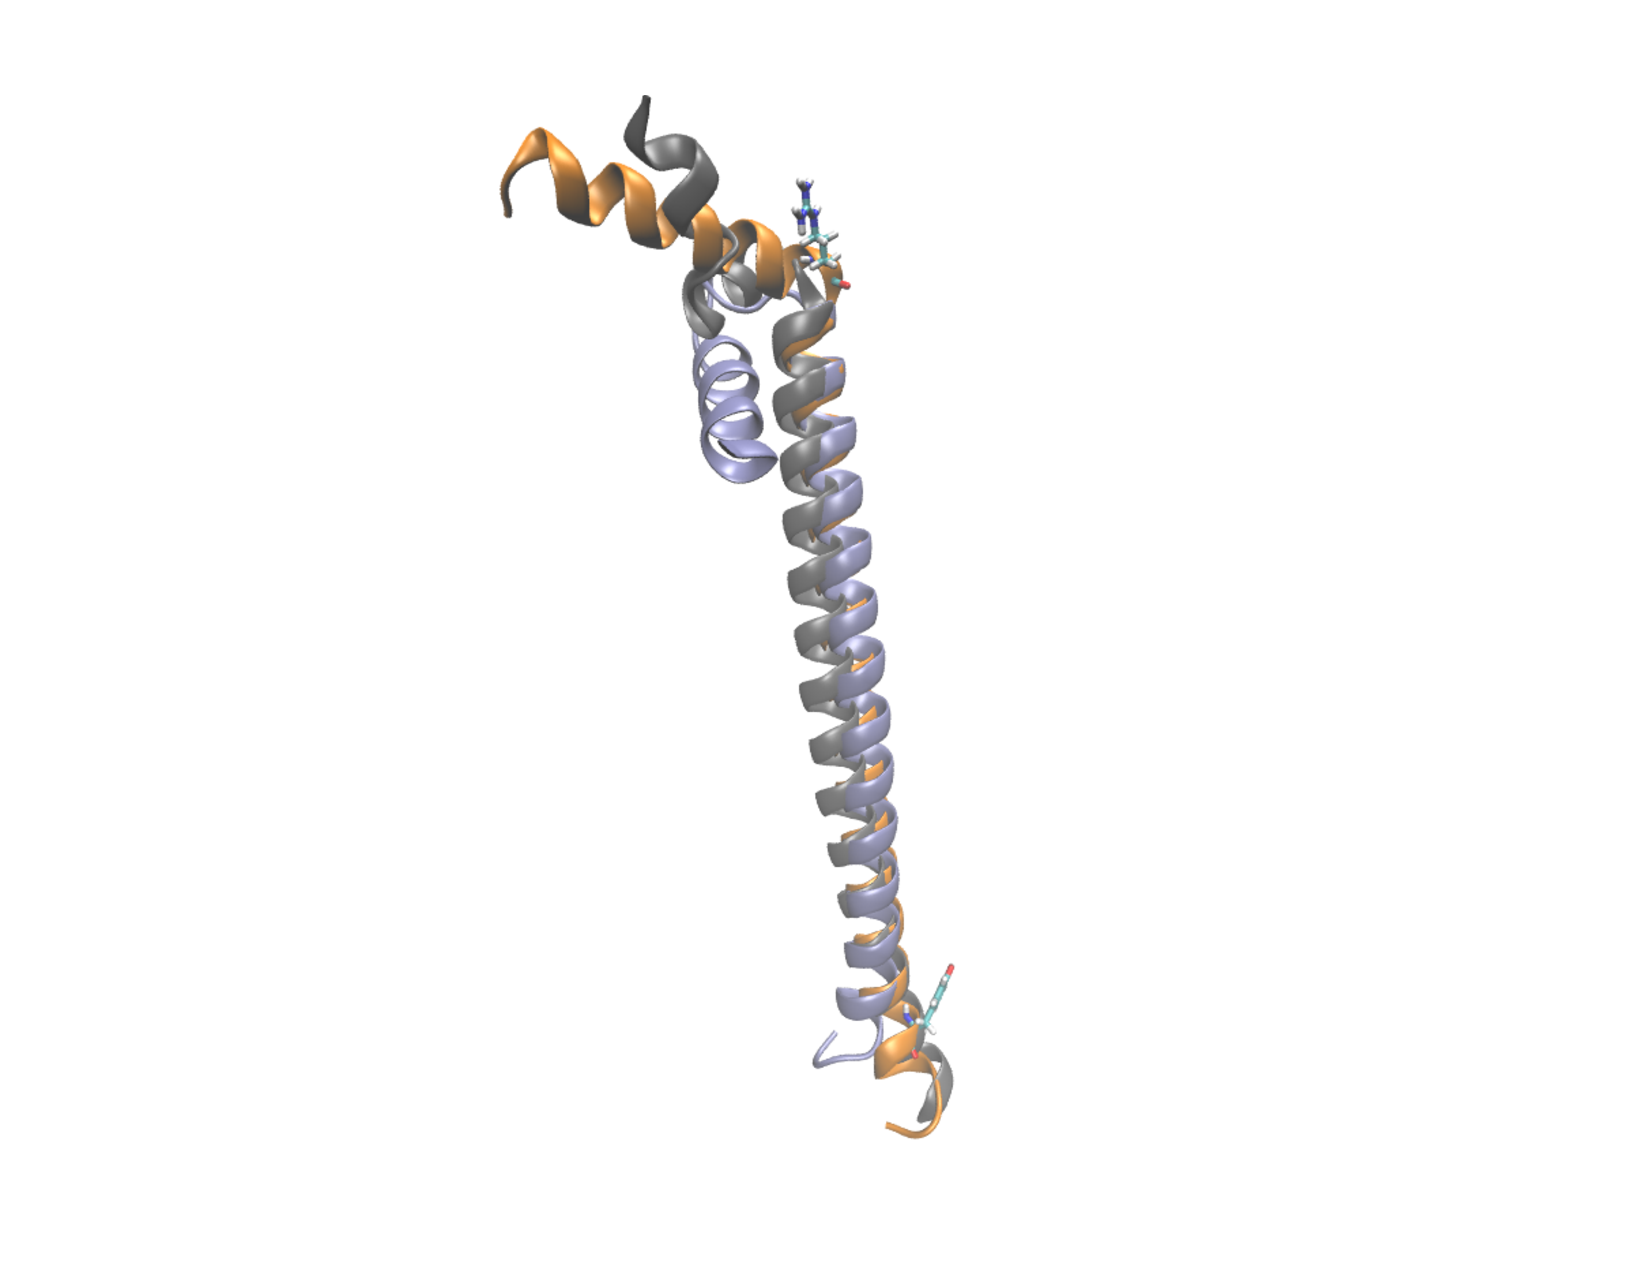
\includegraphics[width=12cm,height=10cm]{T0605.pdf}
\end{center}
\caption{ Three models of the leucine zipper domain of cGMP dependent protein
kinase I (original pdb id: 3NMD and CASP target: T0605). The original target sequence of this protein was 72 residues.
However only residues 3 to 66 is only kept during result announcement as that part can be found from crystallographic analysis. The
region 3 to 66 are almost identical in all the 3 models  }
\label{fig:T0605}
\end{figure}


\begin{thebibliography}{99}

\bibitem{Meirovitch2007}
Meirovitch, H. Recent developments in methodologies for calculating the entropy and free energy of biological systems by computer simulation.
Current Opinion in Structural Biology, 2007, 17, 181-186.

\bibitem{Chipot2007}
Chipot, C.; Shell, M.S.; Pohorille, A. Introduction, in Chipot, C., Pohorille, A., editors. Free Energy
Calculations: Theory and Applications in Chemistry and Biology. Springer Series in Chemical
Physics, vol. 86. Berlin and Heidelberg: Springer; 2007, p. 1–32.

\bibitem{Jorgensen2004}
Jorgensen, W.L. The many roles of computation in drug discovery, Science 2004, 303, 1813–8.

\bibitem{Gilson2007}
Gilson, M.K.; Zhou, H.X. Calculation of protein-ligand binding affinities. Annu Rev Biophys Biomol Struct. (2007) 36, 21-42.

\bibitem{Torrie1977}
Torrie, G. M.; Valleau, J. P. iNonphysical sampling distributions in Monte Carlo free-energy estimation: Umbrella sampling 
(1977) J. Comput. Phys. 23, 187

\bibitem{Tironi1994}
Tironi, I.G.; van Gunsteren, W.F. A molecular-dynamics simulation study of chloroform. Mol. Phys. (1994) 83, 381-403.

\bibitem{Dill1997}
Dill, K.A.; H.S. Chan.  From Levinthal to Pathways to Funnels:  The "New View" of Protein Folding Kinetics.  Nature Structural Biology 4, 10-19 (1997)

\bibitem{Dill2008}
Dill, K.A.; Ozkan, S.B.; Shell, M.S.; Weikl, T.R. The protein folding problem. Annual Review of Biophysics (2008), 37, 289-316.

\bibitem{Anfinsen1973}
Anfinsen. C.B. Principles that Govern the Folding of Protein Chains. Science (1973) 181, 223-230.

\bibitem{Christ2007}
Christ, C.D.; van Gunsteren, W.F. Enveloping distribution sampling: A method to calculate free energy differences from a single simulation,
J. Chem. Phys. (2007), 126, 184110.

\bibitem{Ytreberg2006}
Ytreberg, F.; Zuckerman, D. Simple estimation of absolute free energies for biomolecules. J. Chem. Phys. 2006, 124, 104105.

\bibitem{Park2008}
Park, S.; Lau, A.; Roux, B. Computing conformational free energy by deactivated morphing. J. Chem. Phys. 2008, 129, 134102

\bibitem{Zheng2008}
Zheng, L.; Chen, M.; Yang, W. Random walk in orthogonal space to achieve efficient free-energy simulation of complex systems, Proc. Natl. Acad. Sci. 2008, 105 (51), 20227.

\bibitem{Tyka2006}
Tyka, M.; Clarke, A.; Sessions, R. An Efficient, Path-Independent Method for Free-Energy Calculations. J.Phys.Chem. B 2006, 110, 17212-17220.

\bibitem{Cecchini2009}
Cecchini, M., Krivov, S.V., Spichty, M., Karplus, M. Calculation of free-energy differences by confinement simulations. Application to peptide conformers. 
J. Phys. Chem. B 113, p. 9728-9740 (2009).

\bibitem{Strajbl2000}
Strajbl, M.; Sham, Y.Y.; Villà, J.; Chu, Z.-T.; Warshel, A. Calculations of Activation Entropies of Chemical Reactions 
in Solution. (2000) 104, 4578-4584.  

\bibitem{Krivov2004} 
Krivov, S.; Karplus, M. Hidden complexity of free energy surfaces for peptide (protein) folding Proc. Natl. Acad. Sci. U.S.A. 2004, 101, (41), 14766.

\bibitem{Alexander2007}
Alexander, P.A.; He, Y.; Chen, Y.; Orban, J. Bryan, P. The design and characterization of two proteins with $88 \%$ sequence identity but different 
structure and function. Proc. Natl. Acad. Sci. 2007, 104 (29), 11963-11968.

\bibitem{He2008}
He, Y.; Chen, Y.; Alexander, P.A.; Orban, J. NMR structures of two designed proteins with high sequence identity but different fold and function. Proc. Natl. Acad. Sci. 2008, 105 (38), 14412-14417.

\bibitem{Alexander2009}
Alexander, P.A.; He, Y.; Chen, Y.; Orban, J. Bryan, P. A minimal sequence code for switching protein structure and function. Proc. Natl. Acad. Sci. 2009, 106(50), 21149-21154.

\bibitem{Shortle20009}
Shortle, D. One sequence plus one mutation equals two folds. Proc. Natl. Acad. Sci. 2009, 106(50), 21011-21012. 

\bibitem{Sheffler2009}
Sheffler, W.; Baker, D. RosettaHoles: Rapid assessment of protein core packing for structure prediction, refinement, design, and validation. Protein Science. 2009, 18(1), 229-239.


\bibitem{MacCallum2011}
MacCallum, J.; Pérez, A.; Schnieders, MJ.; Hua, L.; Jacobson, M.P.; Dill, K.A. Assessment of protein structure refinement 
in CASP9. Proteins, 2011, 79, 74-90.

\bibitem{Kryshtafovych2011}
Kryshtafovych, A.; Fidelis, K; and Tramontano, A. Evaluation of model quality predictions in CASP9. Proteins, 2011, 79, 91–106

\bibitem{Zemla2003}
Zemla, A. LGA: a method for finding 3D similarities in protein structures. Nucleic Acids Res 2003, 31, 3370–3374.


\bibitem{Perez2012}
Perez, A.; Yang, Z.; Bahar, I.; Dill, K.A.; MacCallum, J.L.; FlexE: Using Elastic Network Models to Compare Models of Protein Structure. J. Chem. Theory Comput., 2012, 8, 3985-3991. 

\bibitem{Wang2011}
Wang, Q.; Vantasin, K.; Xu, D.; Shang, Y. MUFOLD-WQA: A new selective consensus method for quality assessment in protein structure prediction. 
Proteins, 2011, 79: 185–195. 

\bibitem{Case2005}
Case, D.A.; Cheatham, III, T.E.; Darden, T.; Gohlke, Luo, H.R.; Merz, Jr., K.M.;  Onufriev, A; Simmerling, C.; 
Wang, B.; R. Woods, R. The Amber biomolecular simulation programs. J. Computat. Chem. (20005) 26, 1668-1688.



\end{thebibliography}

\end{document}

